\chapter{Dynamic Force Simulation}

In the previous section the calculations at static conditions were described. However, normally you do not just stand statically in the middle of a slackline. Often you want to do some bouncing or jumping which leads to a significant increase of force on the line. The goal of this section is to calculate those forces and get an idea of the influence of different setup parameters like length, pretension and stretch.

\section{Slackline as a Spring}

The simplest approach is to consider the slackline as a spring that can be described with the same formulas as in the previous section. Together with the following formulas and the formulas described in section \ref{sec:basics} it is easy to calculate the movement of the slackliner and the corresponding force:

\begin{align}
v(t) &= at+v_0 \\
s(t) &= \frac{a}{2}t^2 + v_0 t + s_0 \\
F &= a\cdot m
\end{align}

$a$ is the acceleration, $m$ the mass, $v$ the speed and $s$ the current sag. In a first version of the app the following iterative algorithm was used to simulate the movement of a slackliner: 

\begin{enumerate}
	\item Set the sag of the slackline to the current position of  the slackliner
	\item Calculate the force affecting the slackliner $F = m\cdot g - F_{v,slackline}$
	\item Calculate the acceleration of the slackliner $a = F / m$
	\item Calculate change in speed $\Delta v = a\cdot\Delta t$
	\item Calculate change in position $\Delta s = \frac{1}{2}\cdot a\cdot\Delta t^2 + v\cdot\Delta t$
	\item Calculate the current position and speed of the slackliner $s_{t+1} = s_{t} + \Delta s$, $v_{t+1} = v_{t} + \Delta v$
	\item Repeat steps 2 - 6
\end{enumerate}

However, this approach as some disadvantages. First from a numerical perspective it would be better to describe the movement of the slackliner with a differential equation and use a numerical approximation method for solving. But more important, dynamic measurements have shown that slacklines behave more like a viscoelastic material and not like a simple spring, that leads to a different behavior than shown above. To take this into account a more advanced model has to be used for the simulation.

\section{The Standard Linear Solid Model}

\begin{figure}[htb] \centering
	\includegraphics[width=0.4\textwidth]{images/dynamicStandardModel.pdf}
	\caption{Standard linear solid model}
	\label{fig:dynamicStandardModel}
\end{figure}

The standard linear solid model shown in figure \ref{fig:dynamicStandardModel} is a model to describe the behavior of viscoelastic materials. The springs and damper in the model can be described with the following equations:

\begin{align}
F_{k_1} &= k_1 \cdot x_1 \\
F_{k_2} &= k_1 \cdot x_2 \\
F_{d} &= d \cdot \dot x_2
\end{align}

From the connection of the elements in figure \ref{fig:dynamicStandardModel} follows:

\begin{equation}
	F_{k_1} = F_{k_2} + F_d
\end{equation}

Together with $x_1 + x_2 = x$ and $F = k_1 \cdot x_1$ the following equation can be derived:

\begin{equation}
	F + \frac{d}{k_1 + k_2} \dot F = \frac{k_1 \cdot k_2}{k_1 + k_2} x + \frac{d \cdot k_1}{k_1 + k_2} \dot x
	\label{eqn:linearSolidModel}
\end{equation}

With this equation the behavior of the slackline will be described in the following. For static conditions we have $\dot x_1 = 0$. Therefore the total spring constant $k_{ges} = \frac{k_1 \cdot k_2}{k_1 + k_2}$ can be described by the static stretch behavior of the slackline from the previous chapter with the following formula:

\begin{equation}
	k_{ges} = \frac{1}{\alpha \cdot l}
\end{equation}

So $k_1$ and $k_1$ are determined by the stretch coefficient which is known for many webbings and the ratio $\frac{k_1}{k_2}$ that might be similar on different webbings.

\section{Equation of Motion}

By looking at the equations from section \ref{sec:basics} again and considering that the acceleration of the slackliner has an additional input on the force in the dynamic case the force at the slackline anchor can be described with

\begin{equation}
	F = \frac{\sqrt{s^2 + \frac{l^2}{4}}}{2 \cdot s} \cdot F_{vertical} = \frac{\sqrt{s^2 + \frac{l^2}{4}}}{2 \cdot s} \cdot m\cdot (g - \ddot s)
\end{equation}

From the geometrics of the slackline the absolute stretch of one slackline half can be described with

\begin{equation}
	x = \frac{\Delta l_0}{2} + \sqrt{s^2 + \frac{l^2}{4}} - \sqrt{s_0^2 + \frac{l^2}{4}}
\end{equation}

where $\Delta l_0 = \alpha \cdot F_0 \cdot l$ is the initial stretch of the line due to pretensioning and $s_0$ is the initial sag of a rodeo line (either $\Delta l_0$ or $s_0$ is always zero). Derivating this equations with respect to the time results in the following two equations:

\begin{align}
	\dot F &=  m \cdot (g - \ddot s) \left( \frac{\dot s}{2 \cdot \sqrt{s^2 + \frac{l^2}{4}}} - \frac{\dot s}{s^2} \sqrt{s^2 + \frac{l^2}{4}} \right) - m \dddot s \frac{\sqrt{s^2 + \frac{l^2}{4}}}{2 \cdot s} \\
	\dot x &= \frac{s \cdot \dot s}{\sqrt{s^2 + \frac{l^2}{4}}}
\end{align}

Inserting this equation into equation \ref{eqn:linearSolidModel} from the linear solid model and solving for $\dddot s$ leads to the following equation of motion:

\begin{equation}
\begin{split}
	\dddot s = \frac{k_1 + k_2}{d} \cdot (g - \ddot s) + \frac{2s\dot s}{l_2}\cdot \left(\frac{1}{2 l_2} - \frac{l_2}{s^2} \right) - \insertForSmartphone{\\}\frac{2sk_1k_2}{dml_1} \left(\frac{\Delta l_0}{2} + l_2 - l_1\right) - \frac{2s^2\dot s k_1}{ml_2^2}	
\end{split}
\label{eqn:equationOfEmotion}
\end{equation}

with

\begin{align}
	l_1 &= \sqrt{s_0^2 + \frac{l^2}{4}} \\
	l_2 &= \sqrt{s^2 + \frac{l^2}{4}}
\end{align}

As it can be seen we have a third order non linear differential equation now that can only be solved with numerical algorithms.

\section{Solving the Equation of Motion with the Runge-Kutta-Method }

To solve the equation of motion it has to be transformed into three first order differential equations:

\begin{align}
	\dot s &=G(s,v,a) = v \\
	\dot v &= H(s,v,a) = a \\
	\dot a &= I(s,v,a) = \frac{k_1 + k_2}{d} \cdot (g - a) + \frac{2sv}{l_2}\cdot \left(\frac{1}{2 l_2} - \frac{l_2}{s^2} \right) - \\ &\frac{2sk_1k_2}{dml_1} \left(\frac{\Delta l_0}{2} + l_2 - l_1\right) - \frac{2s^2v k_1}{ml_2^2}	
\end{align}

Now the equation can be solved iteratively with the Runge-Kutta-Method (4th order) with the following formula:

\begin{align}
	s_{t+1} &= s_t + \frac{1}{6} \cdot \Delta t \cdot (M_{1,i} + 2 M_{2,i} +2M_{3,i} +M_{4,i} ) \\ v_{t+1} &= v_t + \frac{1}{6} \cdot \Delta t \cdot (N_{1,i} + 2 N_{2,i} +2N_{3,i} +N_{4,i} ) \\
	a_{t+1} &= a_t + \frac{1}{6} \cdot \Delta t \cdot (O_{1,i} + 2 O_{2,i} +2O_{3,i} +O_{4,i} ) \\
\end{align}

with 

\begin{align}
	M_{1,i} &= G(s_i, v_i, a_i) \\
	M_{2,i} &= G \left(t_i + \frac{1}{2} \cdot \Delta t \cdot M_{1,i}, t_i + \frac{1}{2} \cdot \Delta t \cdot N_{1,i}, t_i + \frac{1}{2} \cdot \Delta t \cdot O_{1,i}\right) \\
	M_{3,i} &= G \left(t_i + \frac{1}{2} \cdot \Delta t \cdot M_{2,i}, t_i + \frac{1}{2} \cdot \Delta t \cdot N_{2,i}, t_i + \frac{1}{2} \cdot \Delta t \cdot O_{2,i}\right) \\
	M_{4,i} &= G \left(t_i + \cdot \Delta t \cdot M_{1,i}, t_i + \cdot \Delta t \cdot N_{1,i}, t_i +\cdot \Delta t \cdot O_{1,i}\right)
\end{align}
\begin{align}
N_{1,i} &= H(s_i, v_i, a_i) \\
N_{2,i} &= H \left(t_i + \frac{1}{2} \cdot \Delta t \cdot M_{1,i}, t_i + \frac{1}{2} \cdot \Delta t \cdot N_{1,i}, t_i + \frac{1}{2} \cdot \Delta t \cdot O_{1,i}\right) \\
N_{3,i} &= H \left(t_i + \frac{1}{2} \cdot \Delta t \cdot M_{2,i}, t_i + \frac{1}{2} \cdot \Delta t \cdot N_{2,i}, t_i + \frac{1}{2} \cdot \Delta t \cdot O_{2,i}\right) \\
N_{4,i} &= H \left(t_i + \cdot \Delta t \cdot M_{1,i}, t_i + \cdot \Delta t \cdot N_{1,i}, t_i +\cdot \Delta t \cdot O_{1,i}\right)
\end{align}
\begin{align}
O_{1,i} &= I(s_i, v_i, a_i) \\
O_{2,i} &= I \left(t_i + \frac{1}{2} \cdot \Delta t \cdot M_{1,i}, t_i + \frac{1}{2} \cdot \Delta t \cdot N_{1,i}, t_i + \frac{1}{2} \cdot \Delta t \cdot O_{1,i}\right) \\
O_{3,i} &= I \left(t_i + \frac{1}{2} \cdot \Delta t \cdot M_{2,i}, t_i + \frac{1}{2} \cdot \Delta t \cdot N_{2,i}, t_i + \frac{1}{2} \cdot \Delta t \cdot O_{2,i}\right) \\
O_{4,i} &= I \left(t_i + \cdot \Delta t \cdot M_{1,i}, t_i + \cdot \Delta t \cdot N_{1,i}, t_i +\cdot \Delta t \cdot O_{1,i}\right)
\end{align}


Unfortunately there are no measurements available characterizing the dynamic behavior of different webbings, so the parameters $\frac{k_1}{k_2}$ and $d$ can only be guessed. However, as a starting point there are some measurements on climbing ropes available at the following webpage (unfortunately in german): \url{http://www.sigmadewe.com/fileadmin/user_upload/pdf-Dateien/SEILPHYSIK.pdf}.
For the ropes tested there the ratio $\frac{k_1}{k_2}$ was always about $3$. The geometry independent damping factor $\delta = d \cdot l$ was varying between $\delta = 4.8 \dots 9\,kN\cdot s$.
